\documentclass[a4paper,12pt,twoside,openright,titlepage]{book}

%Additional packages
\usepackage[utf8]{inputenc}
\usepackage[T1]{fontenc}
\usepackage[dutch,english]{babel}
\usepackage{syntonly}
\usepackage[official]{eurosym}

% Handle images
%\usepackage[graphicx]
\usepackage{graphicx}
\graphicspath{ {./images/}{./styles/} }
\usepackage{float}
\usepackage{wrapfig}

% Handle URLs
\usepackage{xurl}
\usepackage{hyperref}
\hypersetup{colorlinks=true, linkcolor=blue, citecolor=blue, filecolor=blue, urlcolor=blue, pdftitle=, pdfauthor=, pdfsubject=, pdfkeywords=}

% Tables and listings
\usepackage{multirow,tabularx}
\usepackage[table]{xcolor} % Table colors
\usepackage{scrextend}
\addtokomafont{labelinglabel}{\sffamily}
\usepackage{listings}
\usepackage{adjustbox}

% Turn on indexing
\usepackage{imakeidx}
\makeindex[intoc]

% Define colors
\usepackage{color}
\definecolor{ashgrey}{rgb}{0.7, 0.75, 0.71}



% Listing style
\lstset{
  backgroundcolor=\color{ashgrey}, % choose the background color; you must add \usepackage{color} or \usepackage{xcolor}; should come as last argument
  rulecolor=\color{black},         % if not set, the frame-color may be changed on line-breaks within not-black text (e.g. comments (green here))
  frame=single,	                   % adds a frame around the code
  basicstyle=\ttfamily,  % the size of the fonts that are used for the code
  extendedchars=true,    % lets you use non-ASCII characters; for 8-bits encodings only, does not work with UTF-8
  breakatwhitespace=true, % sets if automatic breaks should only happen at whitespace
  breaklines=true,        % sets automatic line breaking
  keepspaces=true,        % keeps spaces in text, useful for keeping indentation of code (possibly needs columns=flexible)
  columns=fullflexible,	  % Make sure no extra spaces are added.
  showstringspaces=false, % if true show spaces in strings adding particular underscores
  showspaces=false        % show spaces everywhere adding particular underscores; it overrides 'showstringspaces'
}



% Uncomment for production
% \syntaxonly

% Style
\pagestyle{headings}

% Turn on indexing
\makeindex[intoc]

% Define document
\author{D. Leeuw}
\title{Linux: Introductie tot de Command Line Interface}
\date{\today\\v.1.0.0}

\begin{document}
\selectlanguage{dutch}

\maketitle

\copyright\ 2020-2025 Dennis Leeuw\\

\begin{figure}

\includegraphics[width=0.3\textwidth]{CC-BY-SA-NC.png}
\end{figure}

\bigskip

Dit werk is uitgegeven onder de Creative Commons BY-NC-SA Licentie en laat anderen toe het werk te kopi\"eren, distribueren, vertonen, op te voeren, en om afgeleid materiaal te maken, zolang de auteurs en uitgever worden vermeld als maker van het werk, het werk niet commercieel gebruikt wordt en afgeleide werken onder identieke voorwaarden worden verspreid.


%%%%%%%%%%%%%%%%%%%
%%% Introductie %%%
%%%%%%%%%%%%%%%%%%%

\frontmatter
\chapter{Over dit Document}
\section{Leerdoelen}
Na het bestuderen van dit document heeft de lezer kennis van:
\begin{itemize}
\item de Linux shell, de syntax, variabelen en quoting
\item de commando's: ls, pwd, whoami, history, mkdir, cd, rmdir,
\item de speciale betekenis van de \textasciitilde
\item de Shell-variabelen: PATH, HOME, USER
\item quotes en escaping
\item FHS - Filesystem Hierarchy Standard
\item Bestands typen
\end{itemize}

Dit document sluit aan op de volgende onderdelen van de LPI:
\begin{itemize}
\item LPI Linux Essentials 010-160 - 6.2.1 Command Line Basics (weight: 3)
\item LPI Linux Essentials 010-160 - 6.2.3 Using Directories and Listing Files (weight: 2)
\end{itemize}

\section{Voorkennis}
Voor een goed begrip van dit document is er geen voorkennis vereist, wel is het van belang dat de lezer een Linux-distributie ge\"installeerd heeft.

%Dit document behandeld Linux voor het middelbaar beroepsonderwijs in Nederland, maar kan breder ingezet worden, daar het gericht is op het behalen van het LPI Linux Essentials examen. De doelgroep is niveau 4 van het MBO, met enige kennis van computers.

\section*{Versienummering}
Het versienummer van elk document bestaat uit drie nummers gescheiden door een punt. Het eerste nummer is het major-versie nummer, het tweede nummer het minor-versienummer en de laatste is de nummering voor bug-fixes.\par
Om met de laatste te beginnen als er in het document slechts verbeteringen zijn aangebracht die te maken hebben met type-fouten, websites die niet meer beschikbaar zijn, of kleine foutjes in de opdrachten dan zal dit nummer opgehoogd worden. Als docent of student hoef je boek niet te vervangen. Het is wel handig om de wijzigingen bij te houden.\par
Als er flink is geschreven aan het document dan zal het minor-nummer opgehoogd worden, dit betekent dat er bijvoorbeeld plaatjes zijn vervangen of geplaatst/weggehaald, maar ook dat paragrafen zijn herschreven, verwijderd of toegevoegd, zonder dat de daadwerkelijk context is veranderd. Een nieuw cohort wordt aangeraden om met deze nieuwe versie te beginnen, bestaande cohorten kunnen doorwerken met het boek dat ze al hebben.\par
Als het major-nummer wijzigt dan betekent dat dat de inhoud van het boek substantieel is gewijzigd om bijvoorbeeld te voldoen aan een nieuw kwalificatiedossier voor het onderwijs of een nieuwe versie van Linux Essentials van de LPI. Een nieuw major-nummer betekent bijna altijd voor het onderwijs dat in het nieuwe schooljaar men met deze nieuwe versie aan de slag zou moeten gaan. Voorgaande versies van het document zullen nog tot het einde een schooljaar onderhouden worden, maar daarna niet meer.

\section*{Document ontwikkeling}
Het doel is door middel van open documentatie een document aan te bieden aan zowel studenten als docenten, zonder dat hier hoge kosten aan verbonden zijn en met de gedachte dat we samen meer weten dan alleen. Door samen te werken kunnen we meer bereiken.\par
Bijdragen aan dit document worden dan ook met alle liefde ontvangen. Let u er wel op dat materiaal dat u bijdraagt onder de CC BY-NC-SA licentie vrijgegeven mag worden, dus alleen origineel materiaal of materiaal dat al vrijgegeven is onder deze licentie.\par
De eerste versie is geschreven voor het ROC Horizon College.

%\begin{flushleft}
\begin{table}[h!]
\centering
\begin{tabularx}{\textwidth}{ |c|c|c|X| }
\hline
	Versienummer &
	Auteurs &
	Verspreiding &
	Wijzigingen\\
\hline
	0.1.0 &
	Dennis Leeuw &
	Wim Onrust &
	Initieel document\\
\hline
	0.2.0 &
	Dennis Leeuw &
	HEITO18IB-A &
	Toegevoegd: versienummering, de shell, begin van werken met bestanden\\
\hline
	0.3.0 &
	Dennis Leeuw &
	&
	Toegevoegd: Werken met bestanden, Everything is a file, Bestandtypen\\
\hline
\end{tabularx}
\caption{Document wijzigingen}
\label{table:1}
\end{table}
\end{flushleft}



%%%%%%%%%%%%%%%%%
%%% De inhoud %%%
%%%%%%%%%%%%%%%%%
\tableofcontents

\mainmatter

% Requires: GUI, DASH
% Provides: ls, pwd, whoami, hostname, history, mkdir, cd, rmdir, ~
% PATH, HOME, USER
\chapter{Waarom de commandline interface?}
De eerste vraag is meestal waarom we de command line zouden gebruiken als we al een grafische interface hebben. Het
meest simpele antwoord is dat Unix van oorsprong alleen maar een command line interface of CLI had. Maar een beter
antwoord is dat een grafische interface veel resources (geheugen en processor) gebruikt en die resources kunnen we
beter inzetten voor de taken die we het systeem geven. Veel Linux machines draaien als servers in een serverruimte en
staan op de achtergrond hun ding te doen, bijvoorbeeld als webserver. Voor die functie is geen grafische interface
noodzakelijk terwijl op een drukbezochte website elk stukje processor of geheugen nodig kan zijn om de website soepel
te laten lopen. Wat we niet nodig hebben installeren we dan ook niet op de machine, dus geen grafische interface.

Daarnaast zal je hopelijk ervaren dat, omdat Linux op de schouders staat van de vele jaren ervaring uit de Unix-wereld,
dat de command line een enorm krachtige interface is om mee te werken. Vaak kan je op de command line dingen sneller en
makkelijker doen dan je in een grafische interface zou kunnen. Wees niet bevreest als dat in eerste instantie niet zo
lijkt. De leercurve kan, zeker als je niet veel ervaring hebt met bijvoorbeeld de command prompt of powershell van Windows, soms erg stijl zijn.


\chapter{Toegang tot de CLI}
Een Linux server die ge\"installeerd is zonder grafische interface heeft op zijn monitor de prompt Login: daar kan je
inloggen als gebruiker. Via de toets combinatie ALT en F1-F6 kan je schakelen naar verschillende consoles zodat je
meerdere keren ingelogd kan zijn.

Als je werkt vanuit een grafische interface kan je gebruik maken van de Terminal of Terminal Emulator applicatie. Deze brengt je bij de command line interface, zie figuur \ref{fig:DashTerminal}

\begin{figure}
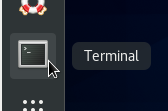
\includegraphics{linuxreader-img021.png}
	\label{fig:DashTerminal}
	\caption{Terminal op de Dash}
\end{figure}


\chapter{De shell}
Alles wat je op de prompt intypt wordt opgevangen door de shell. De shell is een schil rond de kernel die commando's van
gebruikers aanneemt en deze doorgeeft naar de kernel. Shell is het Engelse woord voor schelp en eem schelp zorgt ervoor
dat het weekdier dat in de schelp leeft beschermt wordt tegen de buitenwereld. Dat is bij de shell net zo, de shell
beschermt de kernel tegen de gebruiker. De shell wordt ook wel een command interpreter genoemt omdat hij commando's van
de gebruiker interpreteert.

Linux gebruikt standaard de bash shell. Bijna elke linux distributie levert deze mee en heeft deze als standaard shell.
Van oudsher werd op Unix systemen sh meegeleverd. Het was een van de eerste programma's die werd geschreven voor Unix
door Ken Thompson. Tussen 1976 en 1979 schreef Stephen Bourne een vervanging voor sh wat de standaard werd in Version 7
Unix. De naam bleef echter sh op het Unix systeem. Toen het GNU project een vrij en open source systeem wilde maken was
ook daar een van de eerste programma's die er moest komen een shell. Dat werd bash, de naam bash staat voor Bourne
Again SHell. Het is een open source versie van de shell geschreven door Stephen Bourne.

Unix en Linux commando's en bestandsnamen zijn case sensitive. Dat betekent dat `hello.txt' niet hetzelfde is als
`Hello.txt'. Dit zijn twee verschillende bestanden.

Commando's of opdrachten aan de shell hebben een vaste vorm (syntax). Ze zien er zo uit:

\begin{lstlisting}[language=bash]
commando<spatie>optie(s)<spatie>argument(en)
\end{lstlisting}

De spaties zorgen ervoor dat de shell weet wanneer een volgend deel begint, voor de eerste spatie staat het commando,
daarna volgen er geen of enkele opties en tot slot zijn er geen of enkele argumenten. Bijna alle commando's houden deze
syntax aan, hoewel er natuurlijk uitzonderingen zijn.

Het commando ls laat een lijst met bestanden zien. Als we het gebruiken zonder argumenten dan ziet dat er ongeveer uit als in figuur \ref{fig:lsDir}
\begin{figure}[h]
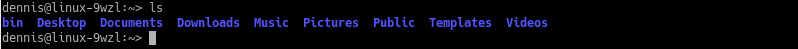
\includegraphics[width=0.9\linewidth]{linuxreader-img023.png}
\label{fig:lsDir}
	\caption{Directory listing}
\end{figure}

Opties worden van argumenten onderscheiden doordat opties beginnen met een min-teken (-). Geven we aan ls een optie me,
bijvoorbeeld -r voor reverse, of wel sorteer omgekeerd dan zien we wat we in figuur \ref{fig:lsRevDir} zien.
\begin{figure}
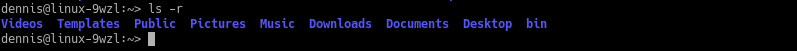
\includegraphics[width=0.9\linewidth]{linuxreader-img024.png}
	\label{fig:lsRevDir}
	\caption{Reverse order listing}
\end{figure}
We zien nu dat Videos vooraan staat en bin achteraan.

We kunnen ook meerdere opties meegeven. De optie -l geeft een long
list, ofwel een lijst die veel meer informatie per bestand of directory laat zien.
\begin{figure}[h]
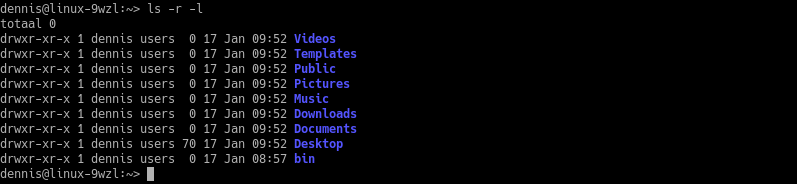
\includegraphics[width=0.9\linewidth]{linuxreader-img025.png}
	\label{fig:lslDir}
	\caption{Reverse and long listing}
\end{figure}
Je mag de opties apart meegeven
zoals we in figuur \ref{fig:lslDir} gedaan hebben maar je mag ze ook samenvoegen zoals:

\begin{lstlisting}[language=bash]
$ ls -lr
\end{lstlisting}
of
\begin{lstlisting}[language=bash]
$ ls -rl
\end{lstlisting}

We kunnen ook een argument meegeven, bijvoorbeeld:
\begin{lstlisting}[language=bash]
$ ls Documents/
\end{lstlisting}
Het argument is de naam van een directory, in dit geval Documents, en we krijgen geen output omdat de directory leeg
is.

De linux shell heeft ook een handigheidje om het leven makkelijker te maken, of beter om minder te hoeven typen, dat
handigheidje heet automatisch aanvullen. Als je op de prompt een p typt zonder een enter te geven en daarna de
tab-toetst indrukt dan gebeurd er niets, druk je nog een keer op de tab-toets dan krijg je de melding:

\begin{lstlisting}[language=bash]
Display all 177 possibilities (y or n)
\end{lstlisting}

Type n want we willen niet 177 mogelijkheden zien. Wat het systeem ons verteld heeft is dat het 177 commando's kent die
met een p beginnen, voegen we nu aan onze p een w toe en typen we 1x tab. Dan vult de shell dit aan met de d en staat
er pwd.

Dit automatische aanvullen kun je doen met commando's maar ook met bestanden en directories. Er wordt weleens gezegd dat
je het toetsenbord van een Linux systeembeheerder kan herkennen aan de versleten tab-toets.


\section{De prompt}
Als je op de command line bent heb je een commandprompt. De commandprompt is het deel voor de cursor, zie \ref{fig:console}

\begin{figure}[h]
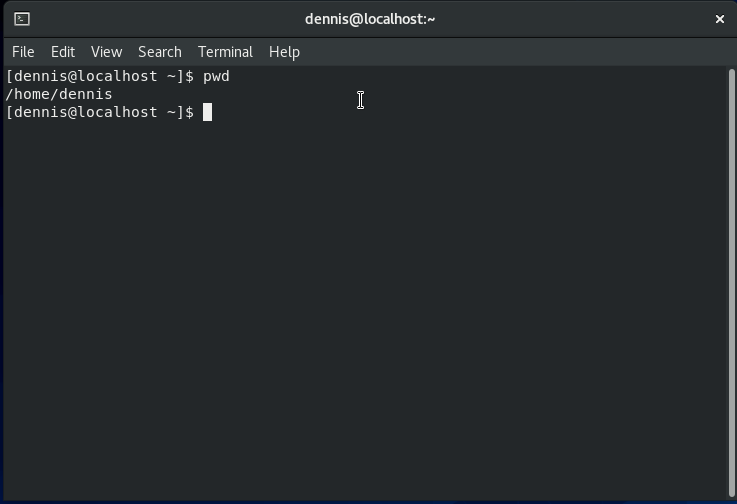
\includegraphics[width=0.8\linewidth]{linuxreader-img022.png}
	\label{fig:console}
	\caption{Console}
\end{figure}

Links staat de login naam, dennis, daarnaast op welke host je bent in gelogd, localhost, daarna volgt de directory
waarin je je nu bevindt, \~{}, en tot slot de prompt voor een normale gebruiker: \$. Als je ingelogt bent als root dan staat er inplaats van een \$ een \#. In deze cursus zullen we alle commando's die je in moet of kan typen op de prompt vooraf laten gaan door een \$ als je het commando als gewone gebruiker moet intypen en door een \# als je het als root moet doen. De \$ en \# moet je dus niet intypen.

Typen we
\begin{lstlisting}[language=bash]
$ pwd
\end{lstlisting}
dan zien we het pad naar de directory waarin we ons bevinden. In dit geval zal dat onze gebruikers
directory zijn met als volledig pad /home/{\textless}gebruikersnaam{\textgreater}. Voor het voorbeeld waarbij de
gebruiker dennis ingelogd is is dat dus /home/dennis. Merk op dat op Linux de directories gescheiden worden door de
forward-slash, /, dit in tegenstelling tot Windows waar de backward-slash, {\textbackslash}, gebruikt wordt als
scheidingsteken.

Nu weten we waar we zijn. Als we willen weten onder welke naam we zijn ingelogd dan gebruiken we
\begin{lstlisting}[language=bash]
$ whoami
\end{lstlisting}
Als je dit commando nu intypt dan zal je je eigen loginnaam zien.

\begin{lstlisting}[language=bash]
$ hostname
\end{lstlisting}
laat zien op welke machine we zitten. Als ik dit commando intyp krijg ik terug `localhost.localdomain', wat
betekent dat mijn machine nog geen echte naam gekregen heeft. Dit kan op je eigen netwerk anders zijn, omdat dit
afhankelijk is van server die de IP-adressen uitdeelt.

\begin{lstlisting}[language=bash]
$ hostname -s
\end{lstlisting}
Geeft alleen de naam van de hostname terug. De -s staat voor short, ofwel kort.

Nu weet je een beetje wie je bent en waar je je bevindt, zowel op welke machine als in welke directory. Welkom thuis.


\section{De home-directory}
Wat waarschijnlijk wat uitleg behoeft is dat je prompt laat zien dat je je in de directory \~{} bevindt. Dat is geen
werkelijk bestaande directory maar een handige afkorting die we binnen de CLI kunnen gebruiken om de home-directory van
een gebruiker aan te duiden. Je eigen plek waar je je bestanden kan opslaan heet je home-directory en die kan dus ook
aangeduid worden met de \~{} (tilde). Je bevindt je dus in je eigen home-directory.

De werkelijke plek waar je je nu bevindt in het bestandssysteem kan je laten zien door
\begin{lstlisting}[language=bash]
$ pwd
\end{lstlisting}
te typen. Het pwd\index{pwd} commando toont de werk-directory en pwd staat dan ook voor print working directory. Je zult zien dat
pwd iets terug geeft als
\begin{lstlisting}[language=bash]
/home/dennis
\end{lstlisting}
waarbij `dennis' vervangen is door je eigen gebruikersnaam. De / (forward slash) is het scheidingsteken dat in Linux
gebruikt wordt om directory namen van elkaar te scheiden. Je bevindt je dus drie directories diep vanaf de root van het
bestandssysteem. / is de root-directory, home/ is de tweede directory en dennis/ is de derde directory.

Laten we eens kijken wat er in onze directory te vinden is. Om een overzicht te krijgen van de directories en bestanden
in onze directory typen we `ls'. `ls' is een afkorting voor list. Ofwel geef een lijst van aanwezige files en
directories. Afhankelijk van de distributie of de systeembeheerder zullen er al wat zaken aanwezig zijn. We gaan er
verder vanuit dat je een standaard CentOS installatie hebt gedaan zoals beschreven in een vorige hoofdstuk.

We gaan onze eerste eigen directory aanmaken. Type hiervoor:
\begin{lstlisting}[language=bash]
$ mkdir LinuxCursus
\end{lstlisting}
met behulp van `ls' kan je zien dat er een nieuwe directory bijgekomen is.

Met `cd', change directory, kunnen we ons verplaatsen in de directory:
\begin{lstlisting}[language=bash]
$ cd LinuxCursus
\end{lstlisting}
na de enter zal je zien dat de prompt gewijzigd is en een `ls' geeft een lege output omdat er
niets in de directory staat. Met `pwd' kan je controleren dat je daadwerkelijk in de nieuwe directory staat.

\begin{figure}
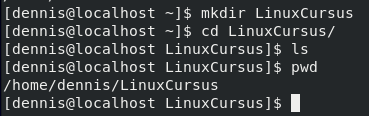
\includegraphics[width=3.8437in,height=1.2083in]{linuxreader-img027.png}
	\label{fig:CreateDirLinuxCursus}
	\caption{Het maken van de LinuxCursus directory}
\end{figure}

Nu gaan we een aantal directories tegelijk aanmaken hiervoor typen we:
\begin{lstlisting}[language=bash]
$ mkdir Data Documenten Muziek
\end{lstlisting}
na een `ls' zie je nu drie nieuwe directories. Zo zie je dat je door meerdere argumenten mee te
geven aan mkdir meer dan 1 directory kan aanmaken.

Met rmdir kan je directories weggooien.
\begin{lstlisting}[language=bash]
$ rmdir Data
\end{lstlisting}
Dit gooit de Data directory weg, na `ls' zie je nu nog maar twee directories.

Als we het systeem verder willen verkennen dan kunnen we met
\begin{lstlisting}[language=bash]
$ cd \~{}
\end{lstlisting}
ervoor zorgen dat we weer in onze home-directory terecht komen, dat scheelt toch een hoop typen die \~{}. \ Als we nu
\begin{lstlisting}[language=bash]
$ cd ..
\end{lstlisting}
typen dan gaan we terug in de directory boom. We komen in de /home/ directory terecht. De dubbele punten naast elkaar
(..) staan voor de directory die 1 stap lager ligt in de boom. We staan nu in de home/ directory die standaard alle
directories van alle gebruikers bevat, dus als er meer gebruikers op het systeem zouden zijn aangemaakt dan zouden ook
van deze gebruikers de home-directories hier te vinden zijn. Een uitzondering is de home-directory van de
systemadministrator van een Linux systeem. Deze beheerder heet `root' en zijn of haar directory is /root/. Daar komen
we later nog een keer op terug.

Als we weer
\begin{lstlisting}[language=bash]
$ cd ..
\end{lstlisting}
typen dan komen we in de / directory terecht. Lager kunnen we niet gaat op een Linux systeem, we zijn nu bij de
root-directory aangekomen. Let op de verwarring die kan ontstaan tussen de /root/ directory en de / directory beiden
heten de root-directory maar de ene is van de gebruiker root en de ander is van het bestandssysteem.

Met alleen het `cd' commando
\begin{lstlisting}[language=bash]
$ cd
\end{lstlisting}
kom je ook weer terug in je eigen home-directory.

\section{History}
Een ander handigheidje van de shell is dat hij een geschiedenis (history) opslaat van gebruikte commando's. Met de
pijltjes toetsen $\uparrow $ (pijltje-omhoog) en $\downarrow $ (pijltje-omlaag) kan je door de geschiedenis van je
commando's scrollen. Omhoog is terug in de tijd en omlaag is het omgekeerde. Met CTRL-c breek je af waar je gebleven
bent en met enter voer je het commando uit.

Met CTRL-r kan je zoeken in je history. Type maar eens CTRL-r en dan de p. Er zal vrijwel direct pwd verschijnen. Op
enter drukken is dan het enige dat nog nodig is om het commando uit te voeren. Als je toch besluit dat je het commando
niet wil uitvoeren dan druk je op CTRL-c om de zoekfunctie te verlaten.

Met !! herhaal je het laatste commando dat je gedaan hebt en met !<commando> herhaal je het
laatste <commando> dat je gedaan hebt. Type nu eens

\begin{lstlisting}[language=bash]
$ !!
\end{lstlisting}

dan zal het pwd commando opnieuw uitgevoerd worden.

\begin{lstlisting}[language=bash]
$ !hostname
\end{lstlisting}
zal de hostname -s uitvoeren want dat is het laatste hostname commando dat we gedaan hebben.

\section{Shell variabelen}
Tot nog toe heb je kennis gemaakt met twee variabelen van de shell. PATH en ?. Er zijn er nog veel meer die standaard beschikbaar zijn. Om er een paar te noemen:
\begin{lstlisting}[language=bash]
$ echo $USER
$ echo $SHELL
$ echo $HOME
$ echo $PWD
\end{lstlisting}
om een complete lijst te krijgen van alle variabelen die in je huidige sessie tot je beschikking staan is er het commando \texttt{env}\index{env}\index{commando!env}.
Als je de waarde van een variabele wil wijzigen gebruik je \texttt{export}\index{export}\index{commando!export}:
\begin{lstlisting}[language=bash]
$ echo $PATH
$ PATH=".:${PATH}"
$ export PATH
$ echo $PATH
\end{lstlisting}
met deze opdracht hebben we de . directory toegevoegd aan de PATH variabele. Als we een commando aanroepen en het komt voor in de directory waar we op dat moment in staan dan zal het dat commando uitvoeren. We hoeven dan niet meer het hele pad of de ./ op te geven.

\section{Eigen variabelen}
Het is soms handig om eigen variabelen te gebruiken:

\begin{lstlisting}[language=bash]
$ aap=1
$ echo $aap
\end{lstlisting}

Zoals je ziet gebruiken we bij het toewijzen van een waarde aan een variable (stop 1 in de variabele aap) geen \$-teken voor de variabele. Alleen bij het gebruik van de variabele zetten we er een \$-teken voor.

Variabelen in de shell hebben ook geen type, er bestaat geen integer of een string, dus we kunnen net zo makkelijk
doen:

\begin{lstlisting}[language=bash]
$ aap="Dag aap!"
$ echo $aap
\end{lstlisting}

het is een goede gewoonte om voor eigen variabelen kleine letters of kleine letter gemixed met hoofdletters te gebruiken en dat variabelen met alleen hoofdletters gereserveerd zijn voor de interne variabelen van de shell.


\section{Shell Quotes en Escapes}
In het hoofdstuk de Shell is de commando syntax uitgelegd. Je hebt daar geleerd dat het commando, de opties en de argumenten geschieden worden door spaties. Stel dat we een directory willen aanmaken met de naam \texttt{Mijn Documenten}. De naam bevat dus een spatie en zou gezien worden als twee argumenten. Om dit op te lossen gaan we gebruik maken van quotes of escape characters en dat is waar deze sectie over gaat.


\subsection{Escapes}
Speciale characters die in de shell al een betekenis hebben kunnen we gebruiken door ze te escapen, van een speciale teken te voorzien. Het escape character in de shell is de \textbackslash, backslash. Voor het maken van een directory of bestand met een spatie erin kunnen we dit doen:
\begin{lstlisting}[language=bash]
mkdir Directory\ met\ spaties
\end{lstlisting}

\subsection{Quotes}
In het vorige hoofdstuk hebben we gezien dat we aan de variable aap een waarde 1 gaven, maar ook de waarde \textquote{Dag aap!}. Bij de ene gebruikten we geen quotes en bij de andere wel. Ook dit had te maken met het gebruik van spaties. Een slimmerik onder jullie zou kunnen zeggen, dan kan je ook een escape gebruiken en dat is helemaal waar, maar stel dat ik het escape-character letterlijk wil nemen en zodat die niet gebruikt wordt als escape, wat dan?

Voer het volgende maar eens uit:
\begin{lstlisting}[language=bash]
$ aap=hello\ world
$ echo $aap
\end{lstlisting}

en nu met quotes:
\begin{lstlisting}[language=bash]
$ aap="hello\ world"
$ echo $aap
\end{lstlisting}

Nu we toch met variabelen aan het spelen zijn, dan kan je ook een variable in een variabele gebruiken zoals hier:
\begin{lstlisting}[language=bash]
$ mies="kees"
$ aap="Hello\ $mies"
$ echo $aap
\end{lstlisting}

Als we mies niet als variabele willen gebruiken dan kunnen we het dollar-teken escapen:
\begin{lstlisting}[language=bash]
$ aap="Hello\ \$mies"
$ echo $aap
\end{lstlisting}
we hebben nu twee escapes in \'e\'en variabele.

We kunnen enkele quotes gebruiken zodat we helemaal geen escapes meer nodig hebben en alles letterlijk wordt weergegeven:
\begin{lstlisting}[language=bash]
$ aap='Hello $mies'
$ echo $aap
\end{lstlisting}
Als we aan aap een complete zin als waarde willen geven kunnen we elke spatie escapen, maar is het korter om enkele quotes te gebruiken.


\section{Opdrachten}

\begin{enumerate}
\item Als ik ingelogd ben als gewone gebruiker met als gebruikersnaam \texttt{karel} en ik type in \texttt{cd \~{}} en ik type daarna \texttt{pwd} wat krijg ik dan als antwoord van de shell?

\item Wat geeft de shell als antwoord na het commando (test het op je eigen systeem):
\begin{lstlisting}[language=bash]
$ echo $PATH
\end{lstlisting}

\item Welk commando gebruiken we om een lege directory weg te gooien?

\item Welke shell gebruiken we op een Linux systeem?

\item In mijn home-directory wil ik een directory met de naam \texttt{Mijn Documenten} maken wat moet ik dan intypen op de prompt om zeker te weten dat deze directory in mijn home-directory aangemaakt wordt?

\item Ga naar de LinuxCursus directory, laat de inhoud van de directory zien en maak een screenshot

\end{enumerate}


\chapter{Het bestandssysteem}
Net als met de standaardisatie van Unix in een POSIX standaard werden er in het begin op Linux Distributies soms bestanden in verschillende directories neergezet. Dat is voor programma's die op die systemen moeten draaien niet handig. Als de ene distributie /var/db heeft voor het plaatsen van databases en de ander /var/databases dan schept dat verwarring. De oplossing die hiervoor gekomen is is de Filesystem Hierarchy Standard. Deze is beschikbaar op \url{https://refspecs.linuxfoundation.org/fhs.shtml}. Hier gaan we heel globaal in op een aantal belangrijke directories, mocht je alle ins en outs willen weten dan raden we je aan om het document een keer te lezen.

\begin{description}
\item [/] De basis van het bestandssysteem wordt bepaald door de root-directory, zo genoemd omdat de vertakkende directories op een boom structuur lijkt en het Engelse root betekend wortel.

Een ls van \texttt{/} laat ons een aantal verschillende directories zien. Waarvan we er een aantal zullen behandelen.

\item [/home/] bevat de directories waarin gebruikers hun bestanden kunnen zetten. Een uitzondering hierop is de directory waarin de root gebruiker (de baas of administrator van het systeem), zijn bestanden kan opslaan. Die directory is \texttt{/root/}.

\item [/etc/] Deze directory bevat de configuratiebestanden van het systeem. Als je een instelling systemwide wilt wijzigen is dit de plek om te gaan zoeken. De configuratie bestanden voor een gebruiker staan in zijn of haar home-directory.

\item [/boot/] Deze directory bevat bestanden die cruciaal zijn voor het opstarten maar die geen commando zijn. Hier vinden we de kernel en bestanden die behoren bij de bootloader.

\item [/dev/] Omdat op een Linus systeem alles een bestand is vind je in deze directory de bestanden die verwijzen aan devices. Devices worden verder besproken in het hoofdstuk over devices. Dus daar gaan we later nog op in.

\item [/var/] is de directory voor de systeem opslag van variabele data zoals bijvoorbeeld de logbestanden, databases, etc. De log bestanden kan je vinden in \texttt{/var/log/}.

\item [/srv/] bevat de data van de diensten die door het systeem worden aangeboden. Data van web- of ftp-servers kan hier gevonden worden.
\end{description}

\section{Everything is a file}
In Unix en Unix-achtige operating systems zoals Linux is het basis principe dat alles een bestand (file) is. Dit betekent dat alles binnen het systeem; documenten, directories, harddisks, printers, toetsenborden, maar ook processen weergegeven worden als bestanden. Het voordeel hiervan is dat dezelfde commando's en API's gebruikt kunnen worden voor verschillende onderdelen van het besturingssysteem.

Het filesysteem is een enkele boom van bestanden en directories, zonder onderscheid tussen disks en partities. Zelfs verplaatsbare media zoals USB-sticks en DVDs zijn onderdeel van deze boom als ze 'gemount' zijn. Ook processen (/proc) en de kernel (/sys) is voor een groot deel benaderbaar via het bestandssysteem.

Met \texttt{ls} kan je in bijvoorbeeld \texttt{/proc} kijken en zien welke processen er zijn. Je ziet er nummers staan en die nummers komen overeen met de process nummers zoals ook \texttt{ps} die heeft. Doe maar eens:
\begin{lstlisting}[language=bash]
$ ps aux
\end{lstlisting}
en je ziet in de tweede kolom dezelfde nummers staan als in \texttt{/proc/}. \texttt{ps} is ook het commando om te zien welke processen er op je systeem actief zijn. We zullen \texttt{ps} in een volgend hoofdstuk uitgebreid behandelen.

\subsection{Bestandstypen}
In de eerste kolom van \texttt{ls -l} vinden we de bestandrechten en het geeft tevens aan met welk type bestand we te maken hebben. Naast normale bestanden (zoals tekstbestanden) hebben we op POSIX-compliant systemen ook speciale bestanden zoals directories.

\begin{center}
\begin{tabular}{ | l | l | c | }
\hline
Bestandstype & Beschrijving & mode veld \\
\hline
\hline
 normaal bestand & Documenten, etc. & - \\
\hline
 directory & Directories bevatten geen bestand, maar een overzicht van de bestandsnamen waaraan gekoppeld referenties naar iets wat inodes worden genoemd. De inodes bevatten de daadwerkelijke bestanden en meta-data (eigenaar, groep, permissies, time stamps, etc.). Door deze manier van werken kan een bestand (met meta-data) verschillende namen hebben (hard-link), mits binnen \'e\'en bestandssysteem (partitie of disk). Bij verschillende bestandsnamen kunnen dezelfde inodes vermeldt staan. & d \\
\hline
 Symbolic link & een link naar een bestand die over bestandssystemen heen kan gaan & l \\
\hline
Block device & Een apparaat waar van of waar naar toe data in een random manier gestuurd kan worden. Het hoeft dus niet in de juiste volgorde te zijn. Denk aan harddisks waar eerst sector 2014 en dan sector 5678 geschreven kan worden. & b \\
\hline
Character device & Een apparaat waar data in een stroom van characters naar of naar toe gestuurd kan worden & c \\
\hline
FIFO & Ook bekend als named pipes. Een pipe verbindt het ene proces met het andere proces zodat data van proces 1 naar proces 2 gestuurd kan worden. Dit kan maar \'e\'en kant op. & p \\
\hline
Socket & Verbindt net als FIFO's processen, maar dan op een manier dat er twee weg communicatie mogelijk is. & s \\
\hline
\end{tabular}
\end{center}


\section{Opdrachten}
\begin{enumerate}
\item Waar kan ik op een Linux systeem de configuratie bestanden vinden?
\item Als ik \texttt{ls -l} gebruik hoe kan ik dan zien of een bestand een directory is?
\item Als er iets niet goed gaat op een Linux systeem in welke directory zou je dan kunnen gaan zoeken naar de fout?
\end{enumerate}



%%%%%%%%%%%%%%%%%%%%%
%%% Index and End %%%
%%%%%%%%%%%%%%%%%%%%%
\backmatter
\printindex
\end{document}

%%% Last line %%%
